\documentclass[aspectratio=169]{beamer}
\makeatletter
\def\input@path{{../common/}{../guide/}{../data/}{../code/}}
\makeatother
\usetheme{Bruno}
\usepackage{amsmath}
\usepackage{amssymb}
\usepackage{siunitx}
\usepackage{float}
\usepackage{tikz}
\def\checkmark{\tikz\fill[scale=0.4](0,.35) -- (.25,0) -- (1,.7) -- (.25,.15) -- cycle;} 
\usepackage{url}
\usepackage[siunitx,american,RPvoltages]{circuitikz}
\ctikzset{capacitors/scale=0.7}
\ctikzset{diodes/scale=0.7}
\usepackage{tabularx}
\newcolumntype{C}{>{\centering\arraybackslash}X}
\renewcommand\tabularxcolumn[1]{m{#1}}% for vertical centering text in X column
\usepackage{tabu}
\usepackage[spanish,es-tabla,activeacute]{babel}
\usepackage{babelbib}
\usepackage{booktabs}
\usepackage{pgfplots}
\usepackage{hyperref}
\hypersetup{colorlinks = true,
            linkcolor = black,
            urlcolor  = blue,
            citecolor = blue,
            anchorcolor = blue}
\usepgfplotslibrary{units, fillbetween} 
\pgfplotsset{compat=1.16}
\usepackage{bm}
\usetikzlibrary{arrows, arrows.meta, shapes, 3d, perspective, positioning,mindmap,trees,backgrounds}
\renewcommand{\sin}{\sen} %change from sin to sen
\usepackage{bohr}
\setbohr{distribution-method = quantum,insert-missing = true}
\usepackage{elements}
\usepackage{verbatim}
\usepackage[edges]{forest}
\usepackage{etoolbox}
\usepackage{schemata}
\usepackage{appendix}
\usepackage{listings}

\definecolor{color_mate}{RGB}{255,255,128}
\definecolor{color_plas}{RGB}{255,128,255}
\definecolor{color_text}{RGB}{128,255,255}
\definecolor{color_petr}{RGB}{255,192,192}
\definecolor{color_made}{RGB}{192,255,192}
\definecolor{color_meta}{RGB}{192,192,255}
\newcommand\diagram[2]{\schema{\schemabox{#1}}{\schemabox{#2}}}

\definecolor{codegreen}{rgb}{0,0.6,0}
\definecolor{codegray}{rgb}{0.5,0.5,0.5}
\definecolor{codepurple}{rgb}{0.58,0,0.82}
\definecolor{backcolour}{rgb}{0.95,0.95,0.92}

\lstdefinestyle{mystyle}{
    backgroundcolor=\color{backcolour},   
    commentstyle=\color{codegreen},
    keywordstyle=\color{magenta},
    numberstyle=\tiny\color{codegray},
    stringstyle=\color{codepurple},
    basicstyle=\ttfamily\footnotesize,
    breakatwhitespace=false,         
    breaklines=true,                 
    captionpos=b,                    
    keepspaces=true,                 
    numbers=left,                    
    numbersep=5pt,                  
    showspaces=false,                
    showstringspaces=false,
    showtabs=false,                  
    tabsize=2
}

\lstset{style=mystyle}
\usepackage{unicode-math}
\setsansfont{Fira Sans}
\setmainfont{Fira Sans}
\setmathfont{Fira Math}

\title{Instrumentación I: \\ \emph{Sensores mecánicos}}
\author{
    Juan J. Rojas
}
\institute{Instituto Tecnológico de Costa Rica}
\date{\today}
\background{background.jpg}
\begin{document}
\sisetup{unit-math-rm=\mathrm,math-rm=\mathrm} % change sinitx font
\sisetup{output-decimal-marker = {,}}
\maketitle

% 6. Transductores mecánicos
% 6.1. Galgas extensiometricas
% 6.2. Celdas de carga
% 6.3. Acelerómetros
% 6.4. Sensores de presión
% 6.5. Velocidad
% 6.6. Giroscopios


\newcommand{\blackandwhite}{white} %change this at the end

\begin{frame}[t]{Deformación unitaria (strain)}
    Cambio en longitud respecto a la longitud original al aplicar una fuerza
    \vspace{0.5cm}
    \begin{equation*}
        \varepsilon = \dfrac{\Delta L }{L_0}
    \end{equation*}
    donde:\\
    $\epsilon$ es la deformación unitaria, adimensional,\\
    $\Delta L$ es el cambio en la longitud después de aplicar la fuerza, y\\ 
    $L_0$ es la longitud original antes de aplicar la fuerza
\end{frame}

\begin{frame}[t]{Esfuezo (stress)}
    Presión interna en un material
    \vspace{0.5cm}
    \begin{equation*}
        \sigma = \dfrac{F}{A}
    \end{equation*}
    donde:\\
    $\sigma$ es el esfuerzo en \si{\newton\meter^{-2}}\\
    $F$ es la fuerza en \si{\newton}, y\\ 
    $A$ es el área trasversal en  \si{\meter^{2}}
\end{frame}

\begin{frame}[t]{Módulo de elasticidad (Young module)}
    Relación entre esfuerzo y deformación en una dirección. Usando esto podemos escribir la Ley de Hooke
    \vspace{0.5cm}
    \begin{equation*}
        \sigma = E\varepsilon
    \end{equation*}
    donde:\\
    $\sigma$ es el esfuerzo en \si{\newton\meter^{-2}}\\
    $E$ es el módulo de elasticidad en \si{\newton\meter^{-2}}, y\\ 
    $\epsilon$ es la deformación unitaria, adimensional,\\
\end{frame}

\begin{frame}{Sensibilidad a la deformación en un resistor}
    En algunos metales y semiconductores la resistencia cambia al ser deformados. Tomando en cuenta que: 
    \begin{equation*}
        R = \rho \dfrac{L}{A}
    \end{equation*}   
    donde: $\rho$ es la resistividad del material en \si{\ohm\meter}, $L$ es la longitud en \si{\meter} y, $A$ es el área trasversal \si{\meter\squared}\\[8pt]
    Si aplicamos el logaritmo y derivamos, obtenemos:
    \begin{equation*}
        \dfrac{\dd R}{R} = \dfrac{\dd \rho}{\rho} + \dfrac{\dd L/A}{L/A}
    \end{equation*} 
    con esto podemos ver que el cambio total tiene una contribucion debido al cambio en la resistividad (efecto piezorresitivo) y otra debido a cambios en la geometría del resistor
\end{frame}

\begin{frame}{Efecto dominante según el material}
    Respecto a la ecuación:
    \begin{equation*}
        \dfrac{\dd R}{R} = \dfrac{\dd \rho}{\rho} + \dfrac{\dd L/A}{L/A}
    \end{equation*} 
    \begin{itemize}
        \item En los metales el efecto dominante es el cambio en la geometría del resistor
        \item En los semiconductores el efecto dominante es el cambio en la resistividad del material
    \end{itemize}
\end{frame}

\begin{frame}[t]{Galgas extensométricas}
    Si integramos los efectos piezorresistivo y geométrico, obtenemos la relación entre la resistencia y la deformación aplicada:
    \begin{equation*}
        \dfrac{dR}{R} = S_s \varepsilon
    \end{equation*}
    donde:\\
    $S_s$ es la sensibilidad o factor de galga, adimensional\\
    $\varepsilon$ es la deformación unitaria, adimensional, y\\
    $R$ es la resistencia en $\si{\ohm}$
\end{frame}

\begin{frame}{Galgas extensométricas: metálica, tipo lámina}
    \begin{columns}[c, onlytextwidth]
        \begin{column}{0.55\textwidth}
            \begin{tabular}{ll}
            \toprule
            \textbf{Parámetro} & \textbf{Valor} \\
            \midrule
            Modelo & BF350-3 AA \\
            Resistencia & \SI{350}{\ohm} \\
            Material base & Fenólico \\
            Espesor & \SI{32}{\micro\meter} \\
            Material res. & constantán \\
            Resistencia aisl. & \SI{10}{\kilo\ohm}\\
            Sensibilidad ($g$) & $2.1 \pm 1\%$\\
            Coeficiente transv & $0.4\%$ \\
            Deformación max & $2.0\%$ \\
            Tamaño ($\si{\milli\meter}$) & $7.1 \times 4.5$ \\
            Temp. oper. & -30$^\circ$C $\sim$ +80$^\circ$C \\
            \bottomrule
            {\footnotesize \href{https://www.elumiled.com/datasheets/BF350-3AA.pdf}{Hoja de datos}}
            \end{tabular}
        \end{column}
        \begin{column}{0.45\textwidth}
        \centering
        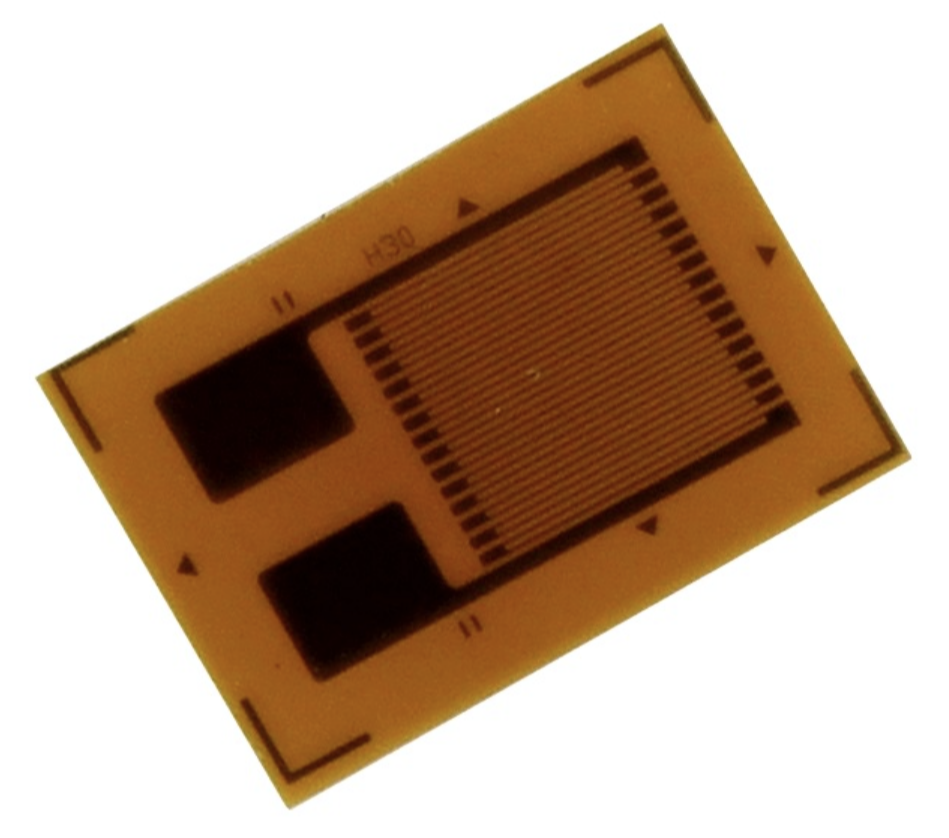
\includegraphics[width = \linewidth]{06_mecánicos/foil_strain_gauge.png}
        \end{column}
    \end{columns}
\end{frame}

\begin{frame}{Galgas extensométricas: metálica, tipo lámina}
    \begin{columns}[c, onlytextwidth]
        \begin{column}{0.60\textwidth}
            La galga BF350-3 AA tiene una sensibilidad $S_s$ de $2.1$ y un coeficiente transversal $k_t$  de $0.4\%$, esto significa que la deformación trasversal $\varepsilon_t$ también afecta la resistencia medida. 
            \begin{equation*}
                \dfrac{dR}{R} = S_s (\varepsilon_l + k_t \varepsilon_t)
            \end{equation*}
            idealmente el coeficiente transversal debe ser lo menor posible, en su defecto, se debe corregir la medición.
        \end{column}
        \begin{column}{0.40\textwidth}
        \centering
        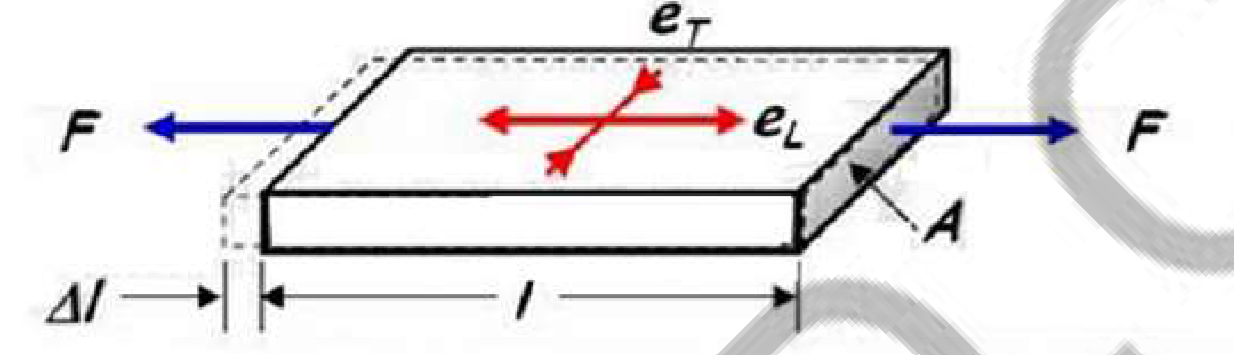
\includegraphics[width = \linewidth]{06_mecánicos/long_trans.png}
        \tiny{Tomado de \href{https://www.elumiled.com/datasheets/BF350-3AA.pdf}{acá}}
        \end{column}
    \end{columns}
\end{frame}

\begin{frame}{Galgas extensométricas: semiconductor}
    \begin{columns}[c, onlytextwidth]
        \begin{column}{0.55\textwidth}
            \begin{tabular}{ll}
            \toprule
            \textbf{Parámetro} & \textbf{Valor} \\
            \midrule
            Resistencia & $\sim$ \SI{10}{\kilo\ohm} \\
            Material base & SiO \\
            Espesor & \SI{10}{\micro\meter} \\
            Material res. & Si \\
            Sensibilidad ($g$) & $103$ c/u\\
            Tamaño ($\si{\micro\meter}$) & $15 \times 300$ \\
            \bottomrule
            \end{tabular}
        \end{column}
        \begin{column}{0.45\textwidth}
            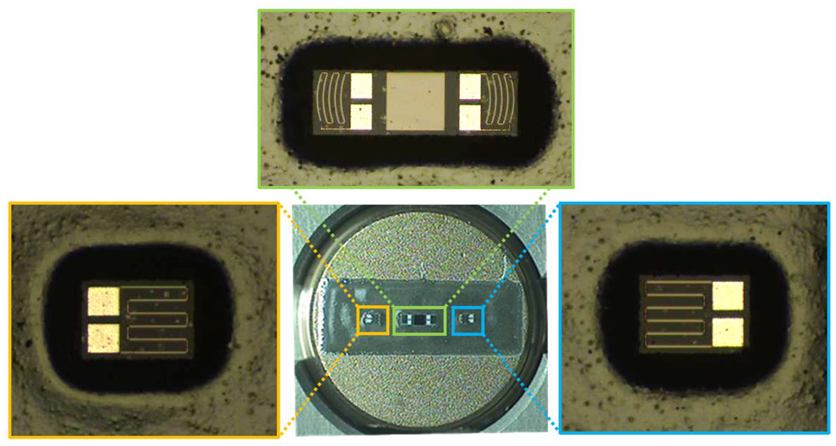
\includegraphics[width = 0.8\linewidth]{06_mecánicos/mems_strain_gauge.png}
            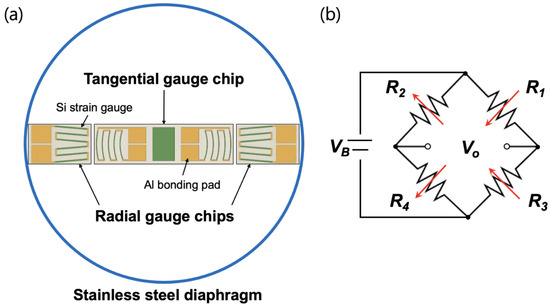
\includegraphics[width = \linewidth]{06_mecánicos/mems_strain_fig.png}

            \tiny{Han, Ji-Hoon, Sung Joon Min, Joon Hyub Kim, and Nam Ki Min. 2023. "Reciprocating Arc Silicon Strain Gauges" Sensors 23, no. 3: 1381. https://doi.org/10.3390/s23031381}
        \end{column}
    \end{columns}
\end{frame}

\begin{frame}{Celdas de carga}
    \begin{columns}[c, onlytextwidth]
        \begin{column}{0.60\textwidth}
            \begin{itemize}
                \item Convierte la deformación mecánica aplicada sobre un elemento elástico en una señal eléctrica proporcional.
                \item Las más comunes utilizan galgas extensiométricas adheridas al elemento elástico.
            \end{itemize}
        \end{column}
        \begin{column}{0.40\textwidth}
            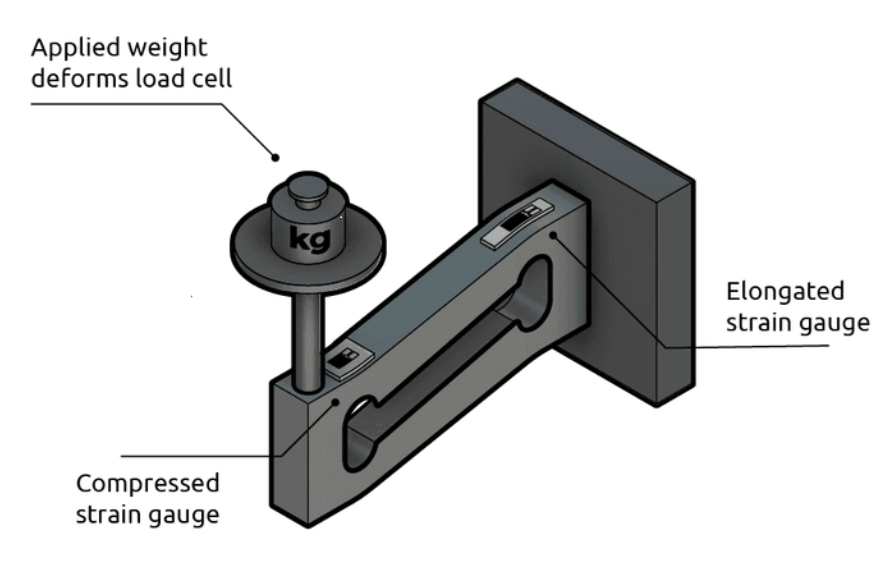
\includegraphics[width = \linewidth]{06_mecánicos/load_cell.png}

            \tiny{Tomado de \href{https://www.flintec.com/}{acá}}
        \end{column}
    \end{columns}
\end{frame}


\begin{frame}{Celdas de carga: aplicaciones}
    \begin{columns}[c, onlytextwidth]
        \begin{column}{0.5\textwidth}
            Algunas aplicaciones comunes de las celdas de carga:
            \begin{itemize}
                \item Medición de fuerza y peso
                \item Medición de presión y nivel
            \end{itemize}
            \centering
            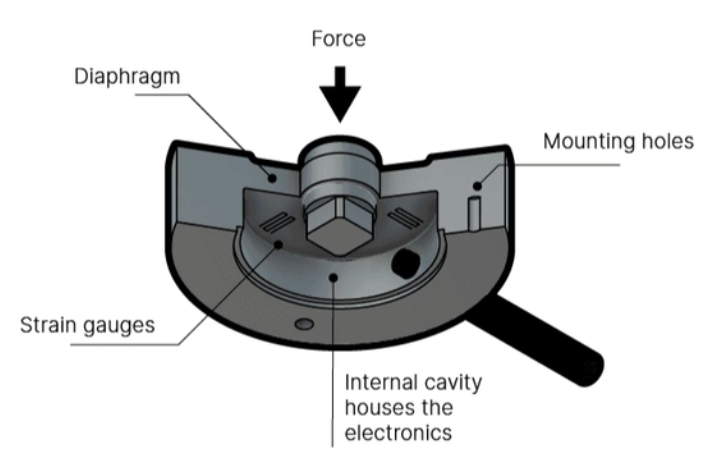
\includegraphics[width = 0.8\linewidth]{06_mecánicos/load_cell_button.png}

            \tiny{Tomado de \href{https://www.flintec.com/}{acá}}
        \end{column}
        \begin{column}{0.5\textwidth}    
            \centering        
            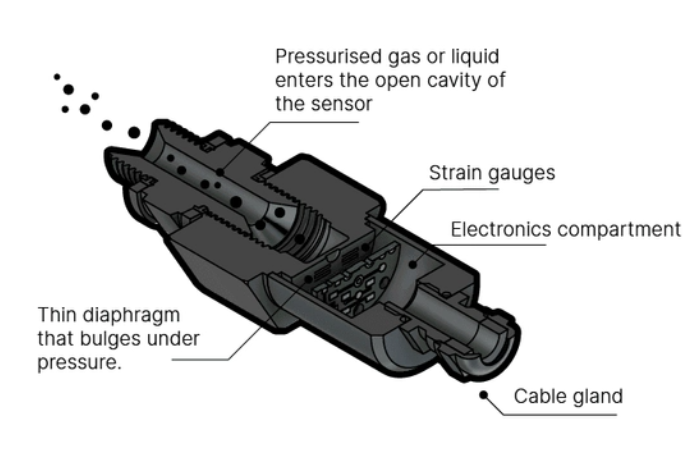
\includegraphics[width = 0.8\linewidth]{06_mecánicos/load_cell_pressure.png}
            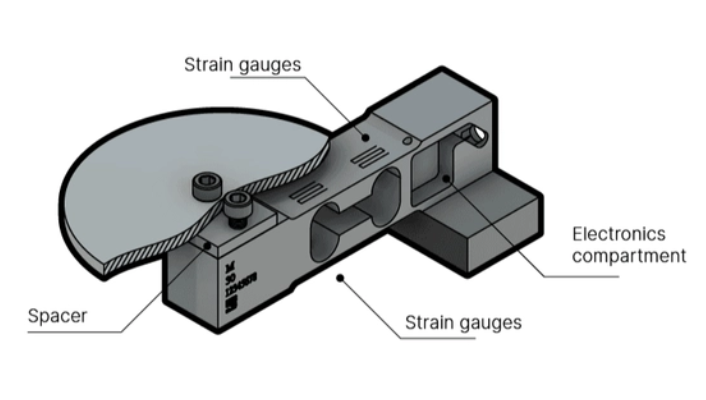
\includegraphics[width = 0.8\linewidth]{06_mecánicos/load_cell_weight.png}
        \end{column}
    \end{columns}
\end{frame}

\begin{frame}{Sensores magnetoelásticos}
    \begin{columns}[c, onlytextwidth]
        \begin{column}{0.6\textwidth}
            \begin{itemize}
                \item La inducción magnética $\mathbf{B}$ y el campo magnético $\mathbf{H}$ están relacionados por:
                \begin{equation*}
                    \mathbf{B} = \mu \mathbf{H}
                \end{equation*}
                donde $\mu$ es la permeabilidad magnética del material en \si{\henry/\meter}
                \item En un sensor magnetoelástico se mide la diferencia en la permeabilidad magnetica del material al ser sometido a una fuerza externa
            \end{itemize}
        \end{column}
        \begin{column}{0.40\textwidth}
            \centering
            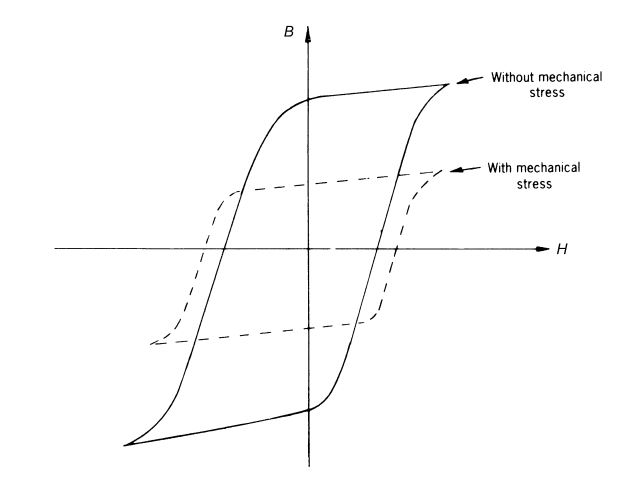
\includegraphics[width = 0.5\linewidth]{Fuerza_Vibracion/magnetoelastico.JPG}
            
            \tiny{Tomado de \cite{pallas2012sensors}}
            
            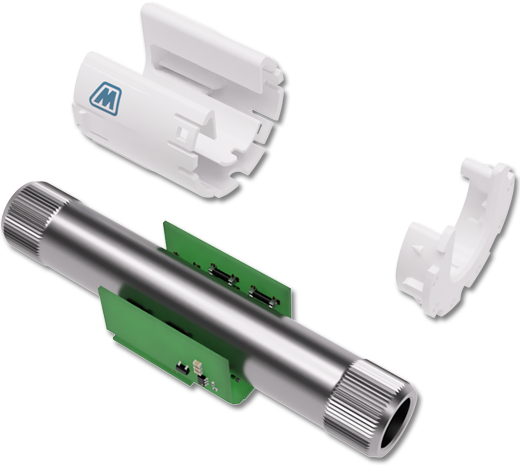
\includegraphics[width = 0.6\linewidth]{Fuerza_Vibracion/Torque-Sensor.png}
            
            \tiny{Tomado de \href{https://www.methodesensor.com/industries/industrial/torque-sensing/}{acá}}
        \end{column}
    \end{columns}
\end{frame}


\begin{frame}{Acelerómetros}
    \begin{itemize}
        \item La vibración es un fenómeno mecánico dinámico en el que existe un movimiento oscilatorio periódico en torno a una posición de referencia 
        \item En algunos casos se puede medir aceleración no vibratoria como la que se obtiene en un impacto o un movimiento lineal
    \end{itemize}
    \begin{columns}[onlytextwidth]
        \begin{column}{0.55\textwidth}
            \begin{itemize}
                \item Los sensores que se utilizan para medir aceleración consisten en un sistema masa resorte amortiguado
                \item El acelerómetro debe ser usado en la parte plana de su curva de respuesta, lejos de su frecuencia natural
            \end{itemize}
        \end{column}
        \begin{column}{0.45\textwidth}
            \centering
            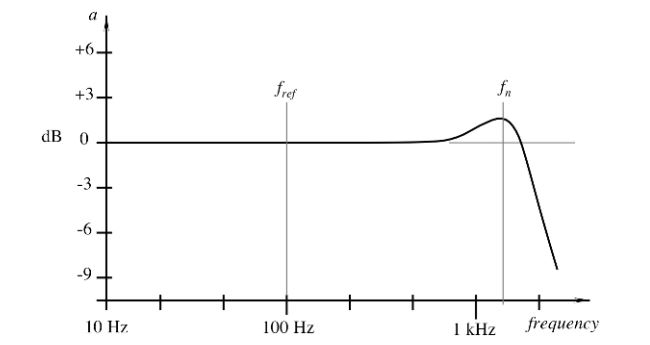
\includegraphics[width = 1\linewidth]{Fuerza_Vibracion/acel.JPG}

            \tiny{Tomado de \cite{Fraden_2016}}
        \end{column}
    \end{columns}
\end{frame}

\begin{frame}{Acelerómetros capacitivos}
    \begin{columns}[c, onlytextwidth]
        \begin{column}{0.65\textwidth}
            \begin{itemize}
                \item Estos sensores consisten de una placa estática y otra placa que esta conectada a una masa inercial, estas dos placas forman un capacitor
                \item La membrana es a su vez la masa inercial, cuando se mueve modifica la capacitancia y esto se relaciona con la aceleración
                \item Típicamente se integran dos capacitores en un solo sensor para incrementar la precisión
                \item A la derecha se muestra su fabricación como sensor MEMS en silicio, con dos capacitores, uno entre la masa el \emph{cap} y otro entre la masa y la \emph{base}
            \end{itemize}
        \end{column}
        \begin{column}{0.35\textwidth}
            \centering
            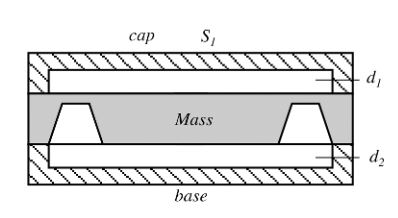
\includegraphics[width = 0.8\linewidth]{Fuerza_Vibracion/memscapacc.JPG}
            
            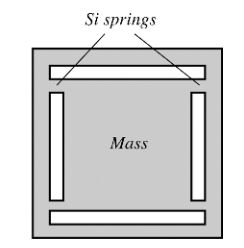
\includegraphics[width = 0.8\linewidth]{Fuerza_Vibracion/memscapacc2.JPG}

            \tiny{Tomado de \cite{Fraden_2016}}
        \end{column}
    \end{columns}
\end{frame}

\begin{frame}{Acelerómetros piezoresistivos}
    \begin{columns}[c, onlytextwidth]
        \begin{column}{0.65\textwidth}
            \begin{itemize}
                \item Estos sensores consisten en galgas extensométricas que miden la deformación en los resortes del sistema masa-resorte
                \item Su precisión es mucho mayor cuando son microfabricados (MEMS)
                \item A la derecha se muestra su fabricación como sensor convencional, cuando la aceleración se aplica sobre el eje sensible la masa inercial gira en torno a la bizagra, al mismo tiempo las galgas experimentan deformación que se relaciona con la aceleración experimentada por la masa inercial
            \end{itemize}
        \end{column}
        \begin{column}{0.35\textwidth}
            \centering
            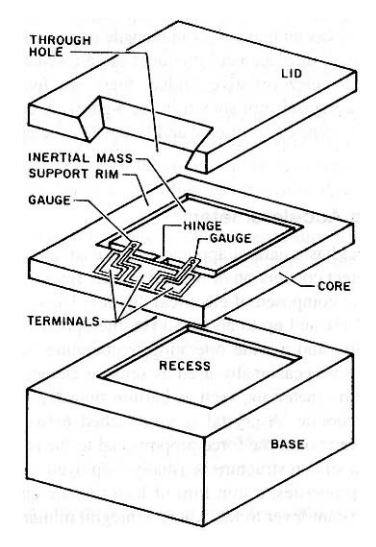
\includegraphics[width = 0.8\linewidth]{Fuerza_Vibracion/memspiezoacc.JPG}
            
            \tiny{Tomado de \cite{Fraden_2016}}
        \end{column}
    \end{columns}
\end{frame}

\begin{frame}{Acelerómetros piezoeléctricos}
    \begin{columns}[c, onlytextwidth]
        \begin{column}{0.6\textwidth}
            \begin{itemize}
                \item Estos sensores consisten de un cristal piezoeléctrico intercalado entre la base y la masa inercial, la fuerza producida por la masa en el piezoeléctrico produce una señal eléctrica entre los electrodos
                \item Es un sensor directo, la energía mecanica se convierte directamente energía eléctrica
                \item Los materiales mas comunes son los materiales ceramicos piezoelectricos como el titanato de bario, el circonato-titanato de plomo (PZT) y la metaniobita de plomo
            \end{itemize}
        \end{column}
        \begin{column}{0.4\textwidth}
            \centering
            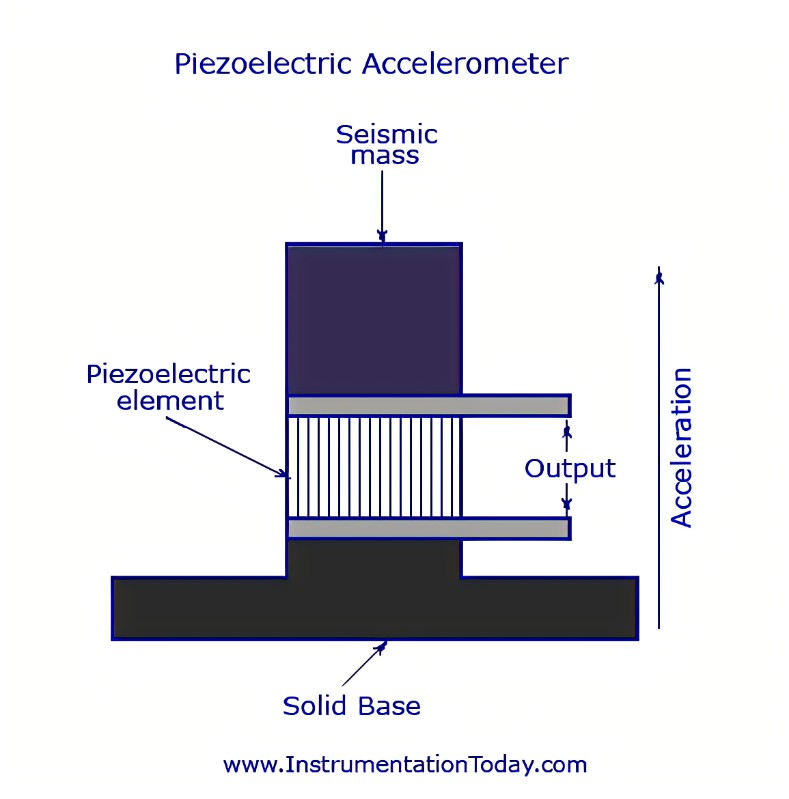
\includegraphics[width = 1\linewidth]{Fuerza_Vibracion/piezo.jpg}
            
            \tiny{Tomado de \href{www.instrumentationtoday.com}{acá}}
        \end{column}
    \end{columns}
\end{frame}

\begin{frame}{Acelerómetros de gas caliente}
            \begin{itemize}
                \item Estos sensores usan un gas caliente como masa inercial
                \item El gas se calienta en el centro del sensor y se mide la temperatura en dos extremos equidistantes, los cambios de temperatura entre los extremos representan aceleración de la masa de gas, pues sin aceleración la distribución de la temperatura debe ser uniforme
                \item Estos sensores son microfabricados (MEMS)
            \end{itemize}
            \centering
            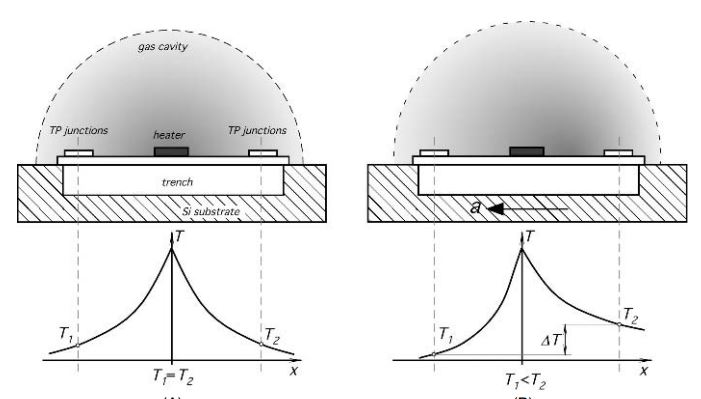
\includegraphics[width = 0.5\linewidth]{Fuerza_Vibracion/memsheatedgasacc.JPG}
            \tiny{Tomado de \cite{Fraden_2016}}
\end{frame}

\begin{frame}{Sensores de presión}
    \begin{columns}[c, onlytextwidth]
        \begin{column}{0.6\textwidth}
            \begin{itemize}
                \item Utilizan un diafragma que se deforma ante de la presión aplicada
                \item La deformación del diafragma se puede medir con galgas extensiométricas, sensores capacitivos, piezoeléctricos o piezorresistivos
            \end{itemize}
        \end{column}
        \begin{column}{0.4\textwidth}
            \centering
            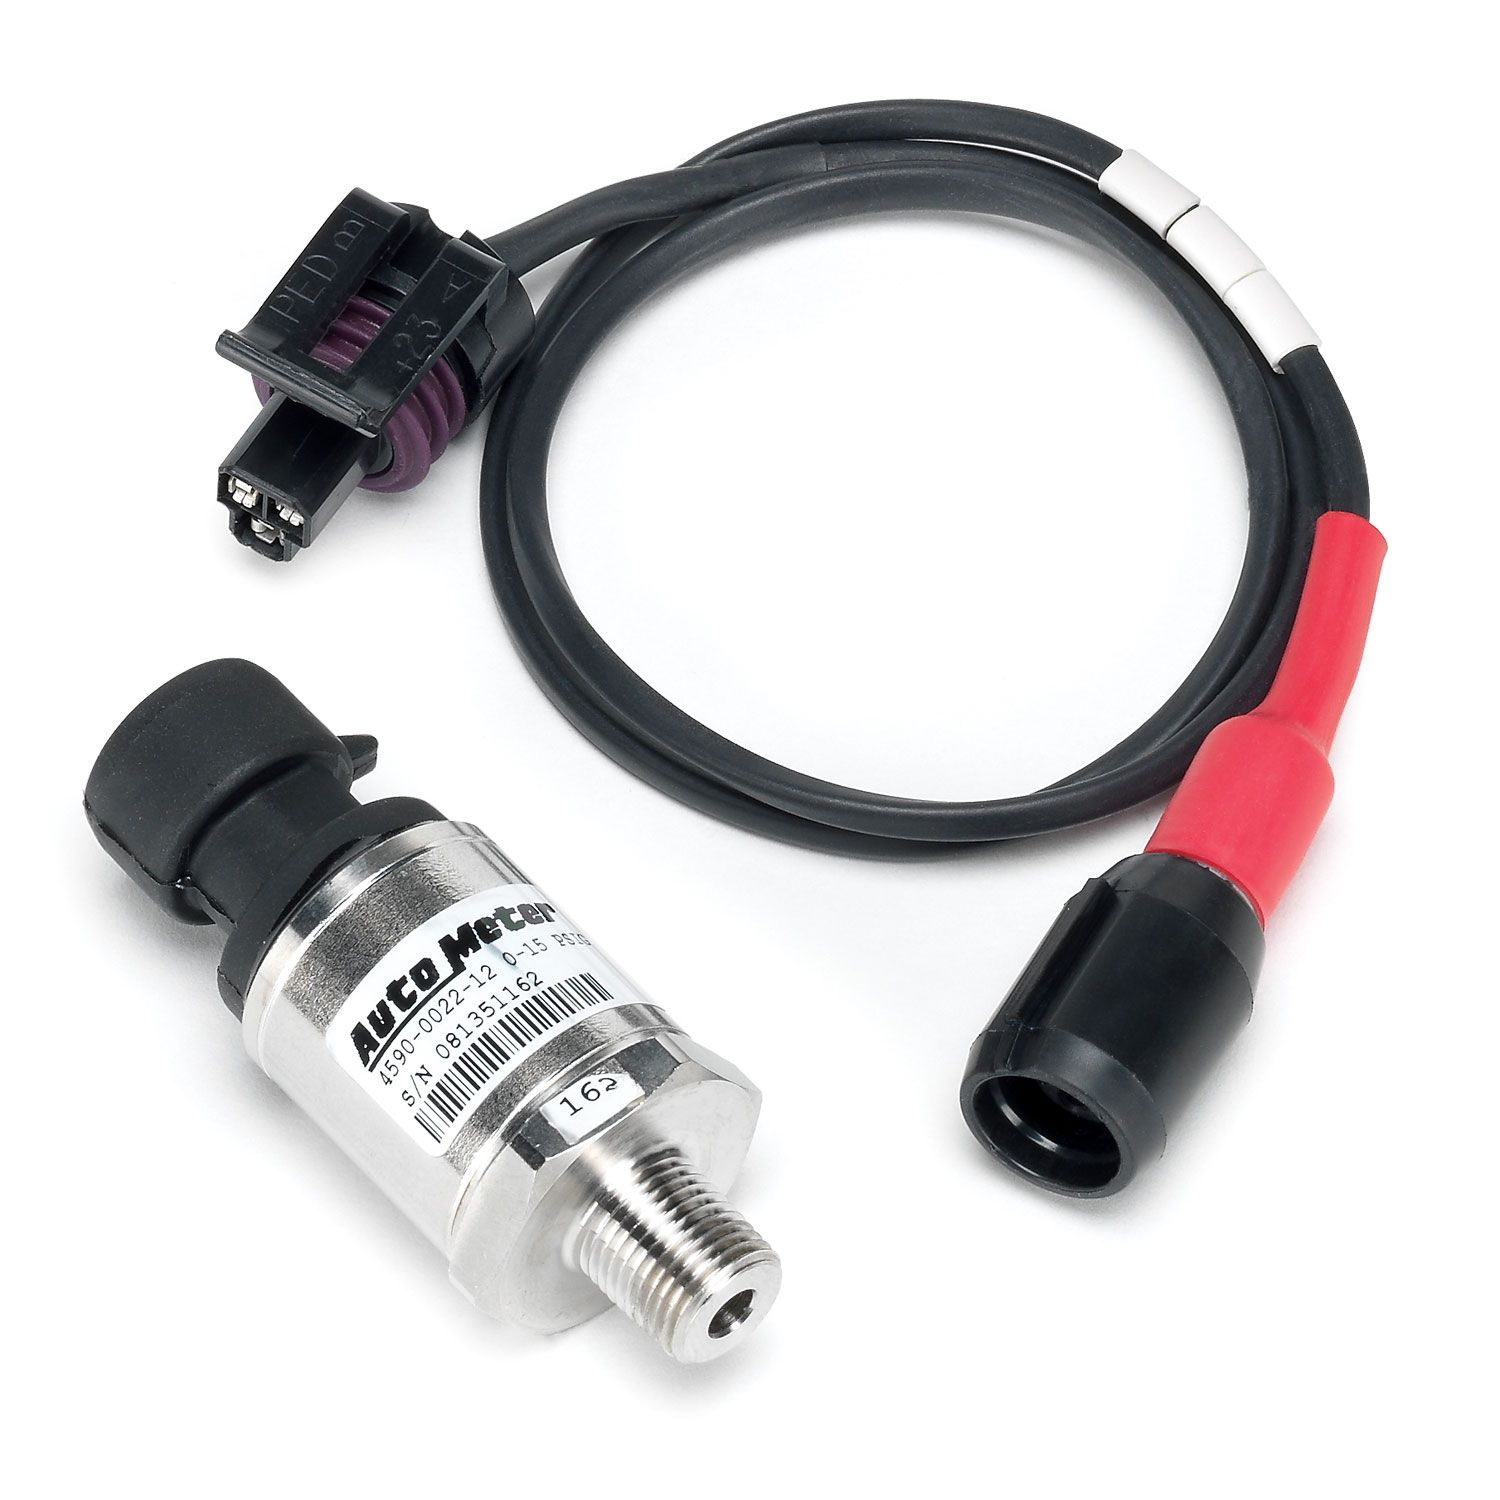
\includegraphics[width = 0.8\linewidth]{06_mecánicos/pressure_sensor.jpg}

            \tiny{Tomado de \href{https://www.processindustryforum.com/article/tips-effective-maintenance-pressure-sensors}{acá}}
        \end{column}
    \end{columns}
\end{frame}

\begin{frame}{Sensores de presión: aplicaciones}
    \begin{columns}[c, onlytextwidth]
        \begin{column}{0.60\textwidth}
            \begin{itemize}
                \item Altitud (cavidad a \SI{101.325}{\kilo\pascal})
                \item Velocidad de un fluido (presión diferencial)
                \item Altura de un tanque (presión hidrostática, diferencial entre el fondo del tanque y el ambiente) 
                \item Presión absoluta (cavidad al vacío)
            \end{itemize}            
        \end{column}
        \begin{column}{0.40\textwidth}
            \centering
            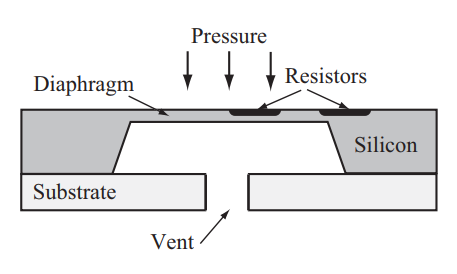
\includegraphics[width = 0.7\linewidth]{06_mecánicos/pressure_piezores.png}
            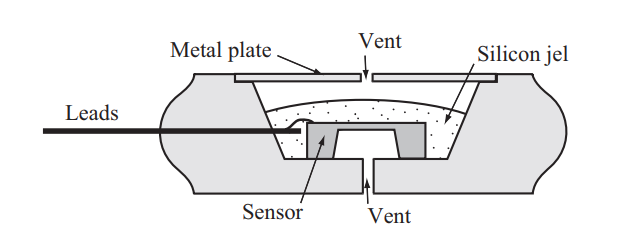
\includegraphics[width = 0.9\linewidth]{06_mecánicos/diff_pressure_piezores.png}
            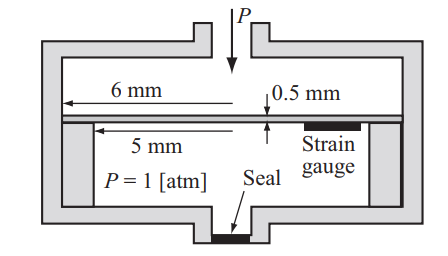
\includegraphics[width = 0.7\linewidth]{06_mecánicos/level_piezores.png}
        \end{column}
    \end{columns}

    \tiny{Tomado de \cite{ida2013sensors}}
\end{frame}

\begin{frame}{Referencias}
\footnotesize
\printbibliography[heading=none]
\end{frame}

\end{document}